% Options for packages loaded elsewhere
\PassOptionsToPackage{unicode}{hyperref}
\PassOptionsToPackage{hyphens}{url}
%
\documentclass[
  12pt,
  a4paper]{extarticle}
\title{Analysis 1B --- Tutorial 10}
\author{Christian Jones: University of Bath}
\date{April 2023}

\usepackage{amsmath,amssymb}
\usepackage{lmodern}
\usepackage{iftex}
\ifPDFTeX
  \usepackage[T1]{fontenc}
  \usepackage[utf8]{inputenc}
  \usepackage{textcomp} % provide euro and other symbols
\else % if luatex or xetex
  \usepackage{unicode-math}
  \defaultfontfeatures{Scale=MatchLowercase}
  \defaultfontfeatures[\rmfamily]{Ligatures=TeX,Scale=1}
\fi
% Use upquote if available, for straight quotes in verbatim environments
\IfFileExists{upquote.sty}{\usepackage{upquote}}{}
\IfFileExists{microtype.sty}{% use microtype if available
  \usepackage[]{microtype}
  \UseMicrotypeSet[protrusion]{basicmath} % disable protrusion for tt fonts
}{}
\makeatletter
\@ifundefined{KOMAClassName}{% if non-KOMA class
  \IfFileExists{parskip.sty}{%
    \usepackage{parskip}
  }{% else
    \setlength{\parindent}{0pt}
    \setlength{\parskip}{6pt plus 2pt minus 1pt}}
}{% if KOMA class
  \KOMAoptions{parskip=half}}
\makeatother
\usepackage{xcolor}
\IfFileExists{xurl.sty}{\usepackage{xurl}}{} % add URL line breaks if available
\IfFileExists{bookmark.sty}{\usepackage{bookmark}}{\usepackage{hyperref}}
\hypersetup{
  pdftitle={Analysis 1B --- Tutorial 10},
  pdfauthor={Christian Jones: University of Bath},
  hidelinks,
  pdfcreator={LaTeX via pandoc}}
\urlstyle{same} % disable monospaced font for URLs
\usepackage[margin=2.5cm]{geometry}
\usepackage{longtable,booktabs,array}
\usepackage{calc} % for calculating minipage widths
% Correct order of tables after \paragraph or \subparagraph
\usepackage{etoolbox}
\makeatletter
\patchcmd\longtable{\par}{\if@noskipsec\mbox{}\fi\par}{}{}
\makeatother
% Allow footnotes in longtable head/foot
\IfFileExists{footnotehyper.sty}{\usepackage{footnotehyper}}{\usepackage{footnote}}
\makesavenoteenv{longtable}
\usepackage{graphicx}
\makeatletter
\def\maxwidth{\ifdim\Gin@nat@width>\linewidth\linewidth\else\Gin@nat@width\fi}
\def\maxheight{\ifdim\Gin@nat@height>\textheight\textheight\else\Gin@nat@height\fi}
\makeatother
% Scale images if necessary, so that they will not overflow the page
% margins by default, and it is still possible to overwrite the defaults
% using explicit options in \includegraphics[width, height, ...]{}
\setkeys{Gin}{width=\maxwidth,height=\maxheight,keepaspectratio}
% Set default figure placement to htbp
\makeatletter
\def\fps@figure{htbp}
\makeatother
\setlength{\emergencystretch}{3em} % prevent overfull lines
\providecommand{\tightlist}{%
  \setlength{\itemsep}{0pt}\setlength{\parskip}{0pt}}
\setcounter{secnumdepth}{5}
\newcommand{\BOO}{BOO}
\usepackage {hyperref}
\hypersetup {colorlinks = true, linkcolor = blue, urlcolor = blue}
\usepackage{float}
\ifLuaTeX
  \usepackage{selnolig}  % disable illegal ligatures
\fi

\usepackage{amsthm}
\theoremstyle{plain}
\newtheorem*{theorem*}{Theorem}\newtheorem{theorem}{Theorem}[section]
\theoremstyle{definition}
\newtheorem*{definition*}{Definition}\newtheorem{definition}{Definition}[section]
\theoremstyle{plain}
\newtheorem*{proposition*}{Proposition}\newtheorem{proposition}[theorem]{Proposition}
\newtheorem*{Definitions*}{Definitions}\newtheorem{Definitions}[definition]{Definitions}
\theoremstyle{plain}
\newtheorem*{lemma*}{Lemma}\newtheorem{lemma}{Lemma}[section]
\theoremstyle{plain}
\newtheorem*{corollary*}{Corollary}\newtheorem{corollary}{Corollary}[section]
\theoremstyle{plain}
\newtheorem*{conjecture*}{Conjecture}\newtheorem{conjecture}{Conjecture}[section]
\theoremstyle{definition}
\newtheorem*{example*}{Example}\newtheorem{example}{Example}[section]
\theoremstyle{definition}
\newtheorem*{exercise*}{Exercise}\newtheorem{exercise}{Exercise}[section]
\newtheorem*{Thought*}{Thought}\newtheorem{Thought}{Thought}[section]
\theoremstyle{remark}
\newtheorem*{remark*}{Remark}
\newtheorem*{solution*}{Solution}
\newtheorem*{Example*}{Example}
\theoremstyle{remark}
\newtheorem*{Proof*}{Proof}
\newtheorem*{Examples*}{Examples}
\let\BeginKnitrBlock\begin \let\EndKnitrBlock\end


%\usepackage[english,shorthands=off]{babel}
\usepackage{etoolbox}
\usepackage{spverbatim}
\makeatletter
\@ifpackageloaded{float}{}{\usepackage{float}}
\@ifpackageloaded{adjustbox}{}{\usepackage[Export]{adjustbox}}
\makeatother
\floatplacement{figure}{H}
\newcommand{\scalefactor}{1.2}
\adjustboxset*{min width=\scalefactor\width,max width=\linewidth}
\renewcommand{\familydefault}{phv}
\fontfamily{phv}\selectfont
\renewcommand{\em}{\bf}\renewcommand{\textit}{\textbf}\renewcommand{\emph}{\textbf}\renewcommand{\it}{\bf}\renewcommand{\itshape}{\bf}
\setlength{\parindent}{0.0pt}
\setlength{\parskip}{1.0\baselineskip}
\renewcommand{\baselinestretch}{1.5}\selectfont
\setlength{\mathsurround}{0.2em}
\setlength{\arraycolsep}{0.5cm}\renewcommand{\arraystretch}{1.5}
\addtolength{\jot}{\baselineskip}
\renewcommand{\;}{\,}
\sloppy
\allowdisplaybreaks
\usepackage{amsthm}
\newtheoremstyle{plain}{20pt}{3pt}{}{}{\bfseries}{.\newline\nobreak}{1.0em\nobreak}{}
\newtheoremstyle{definition}{20pt}{3pt}{}{}{\bfseries}{.\newline\nobreak}{1.0em\nobreak}{}
\newtheoremstyle{remark}{20pt}{3pt}{}{}{\bfseries}{.\newline\nobreak}{1.0em\nobreak}{}
\csundef{Proof}
\csundef{endProof}
\newenvironment{Proof}
  {\noindent{\bf Proof.}\hspace*{1em}}% Begin
  {\qed\par}% End
%% When redefining an environment it is vital that it has 
%% the same number of arguments as the original
\renewenvironment{proof}[1][\proofname]
  {\trivlist\item\relax\noindent{\bf {#1}.}\hspace*{1em}}% Begin
  {\qed\endtrivlist}% End

\begin{document}
\maketitle

{
\setcounter{tocdepth}{2}
\tableofcontents
}
\newpage
\pagenumbering{arabic}

\hypertarget{introduction}{%
\section*{Introduction}\label{introduction}}
\addcontentsline{toc}{section}{Introduction}

Here is the material to accompany the 10th Analysis 1B Tutorial on the 24th April. Alternative formats can be downloaded by clicking the download icon at the top of the page. Please send any comments or corrections to \href{mailto:caj50@bath.ac.uk}{Christian Jones (caj50)}. To return to the homepage, click \href{http://caj50.github.io/tutoring.html}{here}.

\hypertarget{lecture-recap}{%
\section{Lecture Recap}\label{lecture-recap}}

This week is all about making our lives easier! Firstly, we're going to see a criterion for determining whether a function is integrable, and then we're going to see that quite a large class of functions are integrable! Finally, we're going to prime ourselves to develop a well-known result --- the fundamental theorem of calculus --- which links differentiation and integration.

\hypertarget{the-cauchy-criterion-for-integrability}{%
\subsection{The Cauchy Criterion for Integrability}\label{the-cauchy-criterion-for-integrability}}

Recall the definition of the (Riemann) integral:

\BeginKnitrBlock{definition}[Riemann Integral]
{\label{def:def1} }Let \(f:[a,b] \to \mathbb{R}\) be bounded. Then \(f\) is \emph{Riemann integrable} if \[\underline{\int_a^b} f = \overline{\int_a^b} f.\] If this happens, then the (Riemann) integral of \(f\) is defined to be the common value, and given the notation \(\int_{a}^b f.\)
\EndKnitrBlock{definition}

Note that for a function to be integrable, we require both the upper and lower Riemann integrals to exist and be equal. These were defined as follows:

\BeginKnitrBlock{definition}[Lower and Upper Riemann Integrals]
{\label{def:def2} }Let \(f:[a,b] \to \mathbb{R}\) be bounded. Then:

\begin{itemize}
\tightlist
\item
  The \emph{lower Riemann integral} is \[\underline{\int_a^b} f := \sup\left\lbrace L(f,P) \bigg\lvert\; \text{$P$ is a subdivision of $[a.b]$}\right\rbrace.\]
\item
  The \emph{upper Riemann integral} is \[\overline{\int_a^b} f := \inf\left\lbrace U(f,P) \bigg\lvert\; \text{$P$ is a subdivision of $[a.b]$}\right\rbrace.\]
\end{itemize}
\EndKnitrBlock{definition}

To actually find these values, we need to consider \textbf{every} possible subdivision \(P\) of the domain \([a.b]\). Doing this practically is near impossible, except in very rare cases\footnote{Such as the function \(f\) being constant, for example.}. What we would really like is a way of determining integrability from only a selection of partitions. It shouldn't come as a surprise by now that such a method exists, and it's due to --- you guessed it --- Cauchy!\footnote{Result number six on the `named after Cauchy' counter!}

\BeginKnitrBlock{proposition}[Cauchy Criterion for Integrability]
{\label{prp:prop1} }Let \(f:[a,b] \to \mathbb{R}\) be a bounded function. Then \(f\) is Riemann integrable if and only if for all \(\epsilon > 0\), there exists a subdivision \(P\) of \([a,b]\) such that \(U(f,P) - L(f,P) < \epsilon.\)
\EndKnitrBlock{proposition}

So, why is this formulation useful? Due to Archimedes principle, we now only have to consider regularly spaced subdivisions \(P_n\) of \([a,b]\) to determine integrability! In particular, these subdivisions are given by \[P_n = \lbrace x_0, \ldots, x_n\rbrace, \quad x_i = a + \frac{i(b-a)}{n}.\] This criterion also gives us the following theorem:

\BeginKnitrBlock{theorem}
{\label{thm:thm1} }Let \(f:[a,b] \to \mathbb{R}\). Then

\begin{itemize}
\tightlist
\item
  If \(f\) is monotonic, then it is integrable.
\item
  If \(f\) is continuous, then it is integrable.
\end{itemize}
\EndKnitrBlock{theorem}

So, using the Cauchy criterion, we have determined that a large class of functions are integrable! However, to prove the second part of this theorem, we require a (slightly) stronger version of continuity.

\hypertarget{uniform-continuity}{%
\subsection{Uniform Continuity}\label{uniform-continuity}}

Recall the definition of (standard) continuity:

\BeginKnitrBlock{definition}[Continuity]
{\label{def:def3} }Let \(D \subseteq \mathbb{R}\), and \(f: D \to \mathbb{R}\). Then \(f\) is continuous on \(D\) if \[\forall c \in D\;\;\forall \epsilon > 0\;\;\exists \delta = \delta(\epsilon,c) > 0\;\;\text{s.t.}\;\;\forall x \in D,\;\; \lvert x - c \rvert < \delta \Rightarrow \lvert f(x) - f(c) \rvert < \epsilon.\]
\EndKnitrBlock{definition}

In this definition, the `distance' \(\delta\) away from \(c\) you can be for \(f(x)\) to stay within \(\epsilon\) of \(f(c)\) depends on both the choice of \(\epsilon\), and where you are in the domain \(D\), i.e.~your choice of \(c\). If instead, your choice of \(\delta\) remains the same no matter where you are in \(D\), then \(f\) is said to be \textbf{uniformly continuous}. An example of this definition is seen in Figure \ref{fig:unicont}.\footnote{Diagram taken from the \href{https://en.wikipedia.org/wiki/Uniform_continuity}{Wikipedia} page on uniform continuity. The page is really good for extra information too.}

\BeginKnitrBlock{definition}[Uniform Continuity]
{\label{def:def4} }Let \(D \subseteq \mathbb{R}\), and \(f: D \to \mathbb{R}\). Then \(f\) is uniformly continuous on \(D\) if \[\forall \epsilon > 0\;\;\exists \delta = \delta(\epsilon) > 0\;\;\text{s.t.}\;\;\forall x,y \in D,\;\; \lvert x - y \rvert < \delta \Rightarrow \lvert f(x) - f(y) \rvert < \epsilon.\]
\EndKnitrBlock{definition}

\begin{figure}

{\centering 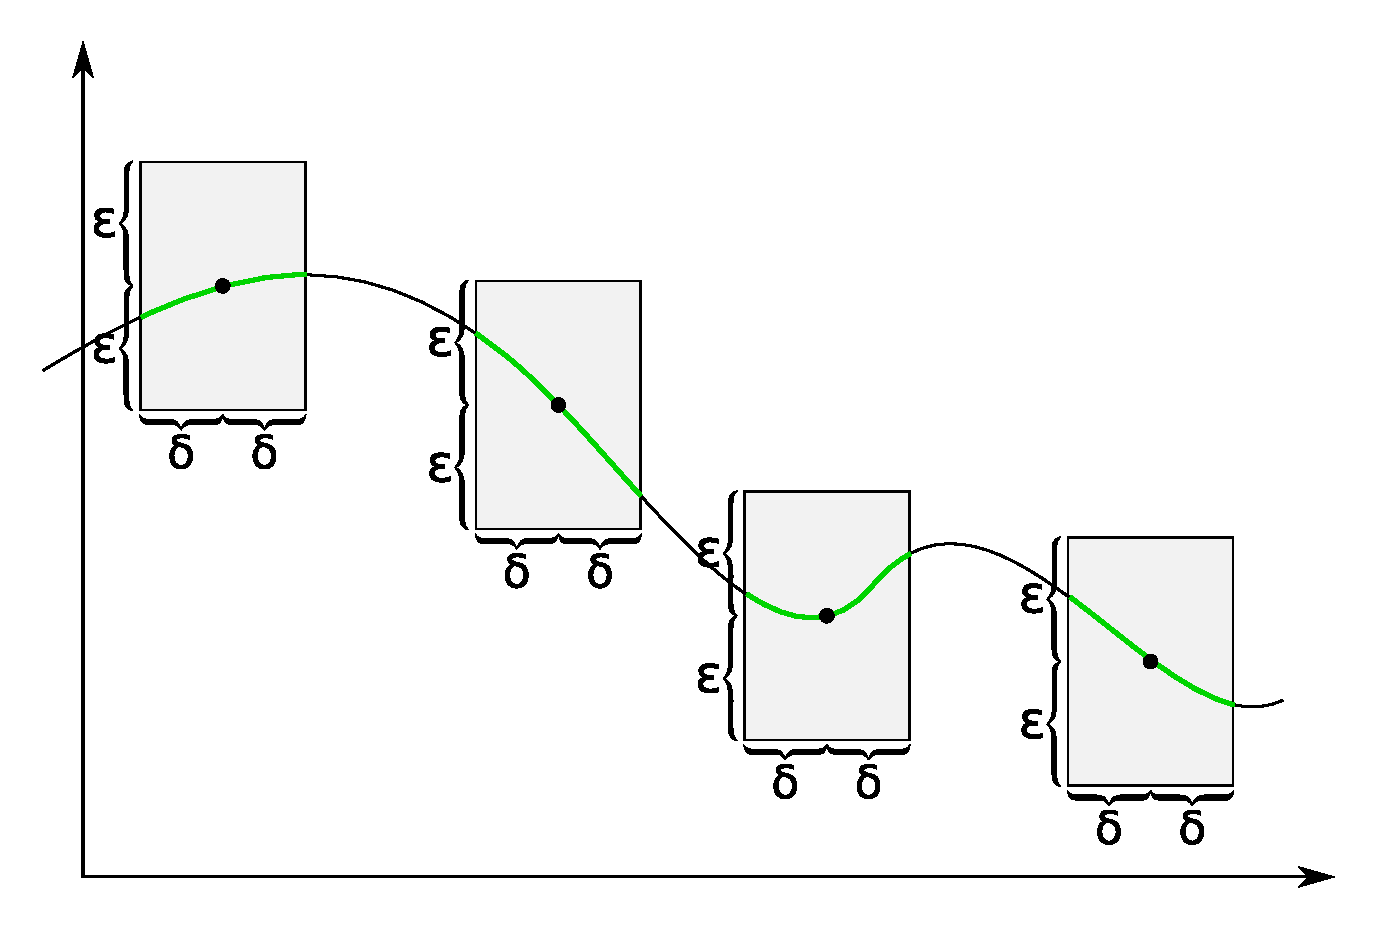
\includegraphics[width=0.5\linewidth]{UniCont} 

}

\caption{An example of a uniformly continuous function. Here, for every $\epsilon > 0$, there exists a $\delta > 0$ such that we can translate a rectangle of width $2\delta$ and height $2\epsilon$ along the function without penetrating the top or bottom edges of the rectangle}\label{fig:unicont}
\end{figure}

Furthermore, from Definition \ref{def:def4}, we see by fixing \(y\), we deduce that if a function is uniformly continuous, it is automatically continuous! In fact, when the function domain is compact (i.e.~think \([a,b]\)), the reverse also holds true:

\BeginKnitrBlock{proposition}
{\label{prp:prop2} }Let \(f:[a,b] \to \mathbb{R}\). Then \(f\) is continuous if and only if it is uniformly continuous.
\EndKnitrBlock{proposition}

\hypertarget{uniform-continuity-and-differentiability}{%
\subsubsection{Uniform Continuity and Differentiability}\label{uniform-continuity-and-differentiability}}

You may remember that if a function \(f:I \to \mathbb{R}\) is differentiable on an open interval \(I \subseteq \mathbb{R}\), then it is continuous on \(I\). However, we cannot strengthen this result in the way you might expect. Namely, it is \textbf{not} true that differentiability implies uniform continuity.

\BeginKnitrBlock{example}
{\label{exm:ex1} }To see why, consider \(f:\mathbb{R} \to \mathbb{R}\) given by \(f(x) = x^2\). We know that the derivative function is \(f':\mathbb{R} \to \mathbb{R}\) given by \(f'(x) = 2x.\) However, f is not uniformly continuous on \(\mathbb{R}\).

To prove this, we consider the negation of the definition, i.e.~we seek \(\epsilon_0 >0\) such that for all \(\delta > 0\), there exists \(x,y \in \mathbb{R}\) such that \(\lvert x - y \rvert < \delta\), and \(\lvert f(x) - f(y) \rvert \geq \epsilon_0.\)

Try \(\epsilon_0 = 1.\) Then
\begin{align*}
\lvert f(x) - f(y) \rvert \geq 1 &\Leftrightarrow \lvert x + y \rvert \geq \frac{1}{\delta}.
\end{align*}

Looking only at positive values of \(x,y\) (which we can do since we are searching for \(x\) and \(y\) in this problem), our two constraints \[\lvert x - y \rvert < \delta \;\; \text{and} \;\; \lvert x + y \rvert \geq \frac{1}{\delta}\] suggest we try \(x = \frac{1}{2\delta}\) and \(y = x + \frac{\delta}{2}.\) Then \[\lvert x - y \rvert = \frac{\delta}{2} < \delta, \;\; \text{and} \;\; \lvert x + y \rvert = \frac{1}{\delta} + \frac{\delta}{2} \geq \frac{1}{\delta}.\] So, we have found an \(\epsilon_0>0\) such that for any positive \(\delta\), we have found \(x,y\) with \(\lvert x - y \rvert < \delta\), and \(\lvert f(x) - f(y) \rvert \geq \epsilon_0.\) This shows that \(f\) is not uniformly continuous.
\EndKnitrBlock{example}

However, all hope is not lost. In fact, using the Mean Value Theorem, we can recover a result linking differentiability and continuity!

\BeginKnitrBlock{proposition}
{\label{prp:prop3} }Let \(f:[a,b] \to \mathbb{R}\) be continuous on \([a,b]\) and differentiable on \((a,b).\) If \(f\) is differentiable on \((a,b)\) with bounded derivative, i.e.~\(\exists L > 0\) such that \(\lvert f'(x) \rvert < L \;\;\forall x \in (a,b)\), then \(f\) is uniformly continuous.
\EndKnitrBlock{proposition}

\hypertarget{other-forms-of-continuity}{%
\subsubsection{Other forms of Continuity}\label{other-forms-of-continuity}}

Whilst less relevant to this course, there are versions of continuity which are stronger still! The first we will mention here is known as Hölder continuity.

\BeginKnitrBlock{definition}[Hölder Continuity]
{\label{def:def5} }Let \(f:D \to \mathbb{R}\), and \(\alpha>0\). Then \(f\) is said to be \(\alpha\)-Hölder continuous if \(\exists L > 0\) such that \(\forall x,y \in D\): \[\lvert f(x) - f(y) \rvert < L \lvert x - y \rvert^{\alpha}.\] The set of all \(\alpha\)-Hölder continuous functions from \(D\) is denoted by \(C^{0,\alpha}\left(D\right).\)
\EndKnitrBlock{definition}

Ok, this definition looks a little complicated, so a visual such as Figure \ref{fig:Holder} is probably quite welcome here for some geometric intuition.

\begin{figure}

{\centering 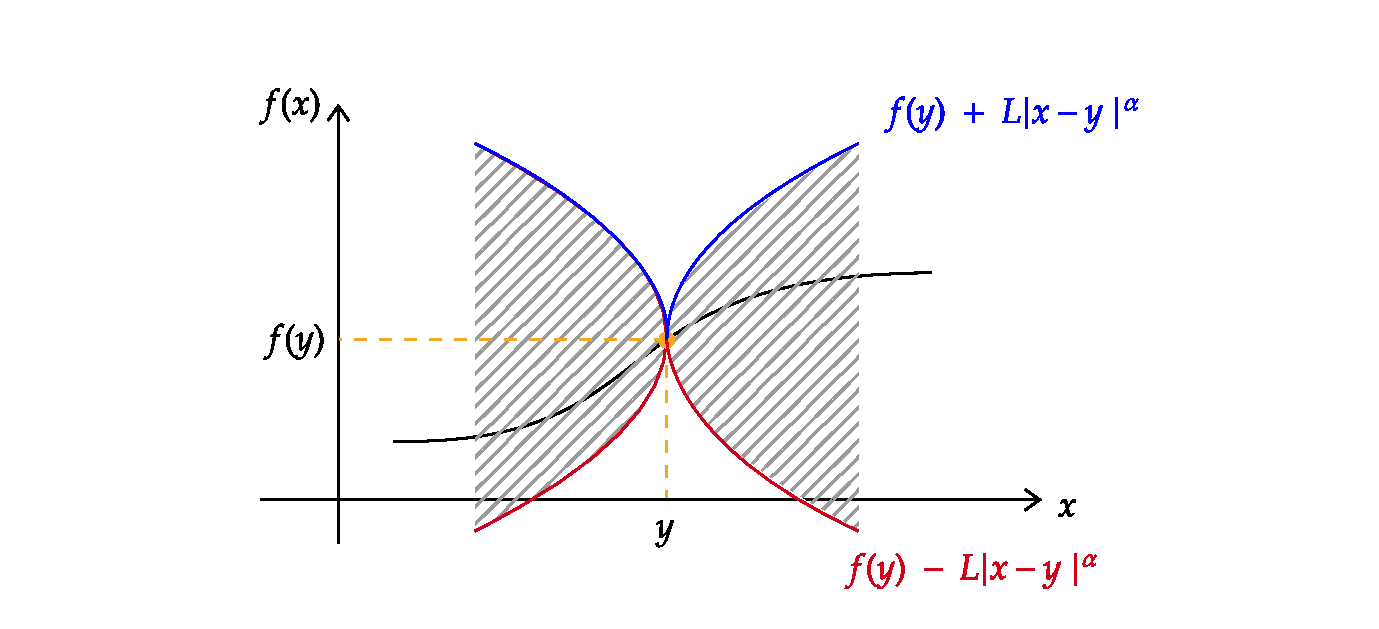
\includegraphics[width=\Width,height=\Height]{Holder} 

}

\caption{An example of a Hölder continuous function. In this case, there exists constants $L$ and $\alpha$ such that we can translate a double parabola along the function in a way that the function remains within the shaded areas.}\label{fig:Holder}
\end{figure}

You've already shown in a previous problem sheet that if \(D\) is an interval, and \(\alpha > 1\), then the only \(\alpha\)-Hölder continuous functions are constant. Another important class of Hölder continuous functions occurs when \(\alpha = 1.\) This is a case you're also likely to have come across in the problem sheets:

\BeginKnitrBlock{definition}[Lipschitz Continuity]
{\label{def:def6} }Let \(f:D \to \mathbb{R}\). Then \(f\) is said to be Lipschitz continuous if \(\exists L>0\) such that \(\forall x,y \in D\): \[\lvert f(x) - f(y) \rvert < L \lvert x - y \rvert.\]
\EndKnitrBlock{definition}

Again, this is something we can visualise (see Figure \ref{fig:Lipschitz}). Quite handily, if we introduce \(\delta = \epsilon/L\), we see that a Lipschitz continuous function satisfies the definition of uniform continuity, and so is also continuous!

\begin{figure}

{\centering 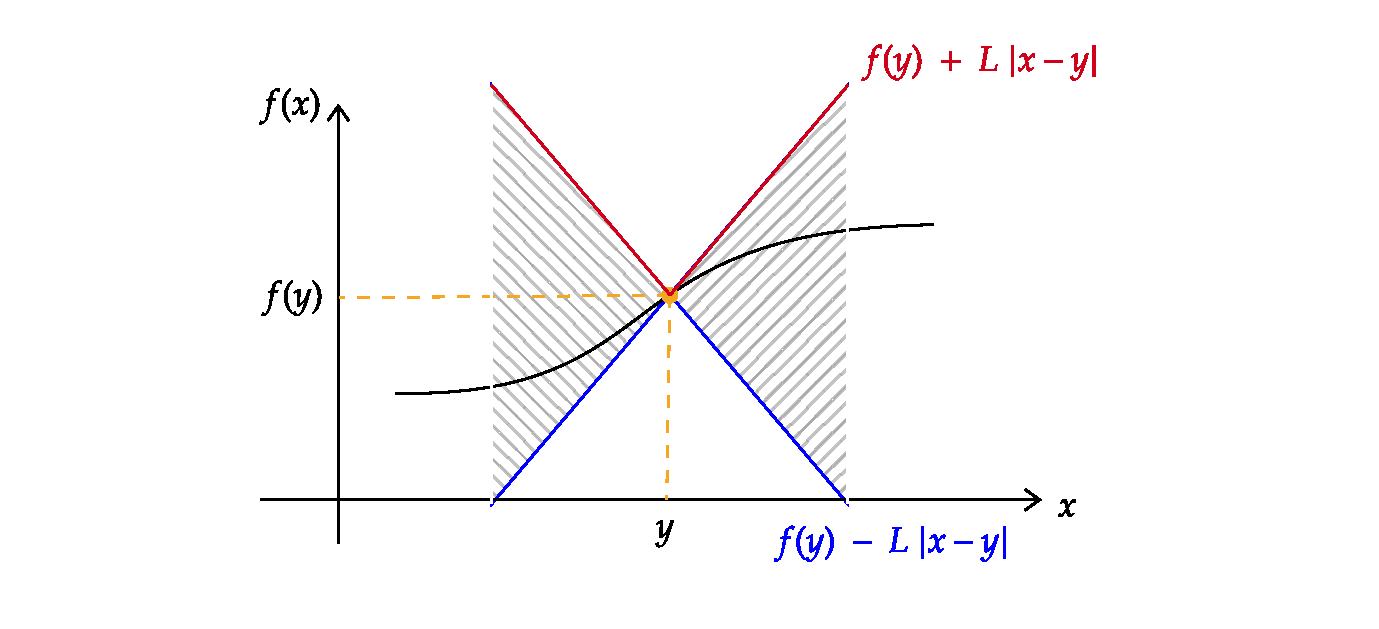
\includegraphics[width=\Width,height=\Height]{Lipschitz} 

}

\caption{An example of a Lipschitz continuous function. In this case, we can translate a double cone along the function, so that the function remains in the shaded area. }\label{fig:Lipschitz}
\end{figure}

\hypertarget{hints}{%
\section{Hints}\label{hints}}

As per usual, here's where you'll find the problem sheet hints!

\begin{enumerate}
\def\labelenumi{\arabic{enumi})}
\tightlist
\item
  The ideas in this one are pretty similar to `Tutorial Question 1'. Here's a potential route through this question:

  \begin{enumerate}
  \def\labelenumii{\alph{enumii})}
  \tightlist
  \item
    Since \(f\) and \(g\) are integrable, they are bounded. So, there exists a common \(M>0\) such that \(\lvert f(x) \rvert \leq M\) and \(\lvert g(x) \rvert \leq M\) for all \(x \in [a,b]\). Why does this mean that \(f\cdot g\) is bounded?
  \item
    Let \(P = \{x_0, \ldots x_n\}\) be a subdivision of \([a,b]\). For any interval \(I_i = [x_{i-1},x_{i}]\), use techniques/results from `Tutorial Question 1' to show that \[\sup_{I_i}(f\cdot g) - \inf_{I_i}(f\cdot g) \leq M(\sup_{I_i}f - \inf_{I_i}f) + M(\sup_{I_i}g - \inf_{I_i}g).\]
  \item
    Using the above result, find a corresponding inequality relating lower and upper Riemann sums.
  \item
    Fix \(\epsilon >0\), and apply the Cauchy criterion to \(f\) and \(g\) separately (obtaining subdivisions \(P_1\) and \(P_2\) respectively). Using these, find a common subdivision for which \(f\) and \(g\) satisfy the Cauchy criterion, and show that with this subdivision, \(f\cdot g\) also satisfies the Cauchy criterion.
  \end{enumerate}
\item
  Firstly, why is \(f\) uniformly continuous on \([0,1]\)? Next, use the definitions for uniform continuity of \(f\) on \([0,1]\) and \(g\) on \([1,\infty)\) to find a candidate \(\delta\) for uniform continuity of \(h\) on \([0,\infty)\). Finally, with this \(\delta\), show that \(h\) satisfies the definition of uniform continuity (you'll need three cases for the values of \(x,y\) in the definition).
\end{enumerate}

\end{document}
